\begin{document}
\sectiontitle{8}{Knee Angle Estimation}
\setstretch{1.6}

Feedback for the closed-loop control system was designed to rely on the knee angle, resulting in the necessity of a robust method of extracting the knee angle from the IMU measurements. This realized by mounting one IMU on the shank and one on the thigh, as can be seen in figure \ref{fig:clsetupimg}. The angle between these two segments could then be calculated using the relative orientation of the IMUs. However, determining this angle requires an algorithm capable of providing accurate, low-latency orientation estimates. 


\subsection{Methods}
\subsubsection{Wireless IMU Integration}
\begin{wrapfigure}{r}{0.5\textwidth}
        \centering
    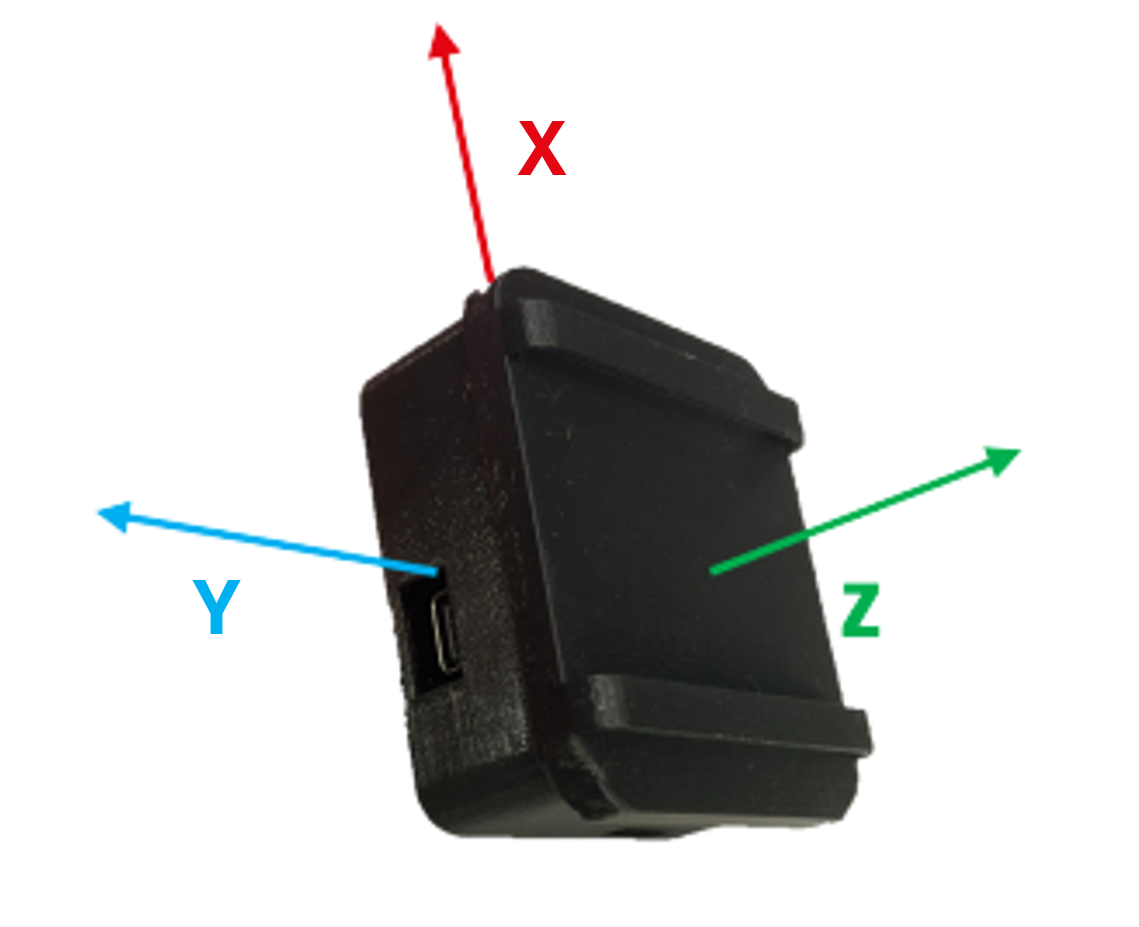
\includegraphics[width=\linewidth]{images/IMU_directions.png}
    \caption{New wireless IMU}
    \label{fig:imudirection}
\end{wrapfigure}
A part of the project involved replacing the old wired IMUs used by the previous student, with new wireless IMUs developed at the laboratory. These new IMUs enhance the portability and adaptability of the system, making them better suited for this application. They feature a high sampling frequency of 1kHz, and are capable of communicating using the Lab Streaming Layer (LSL) protocol. LSL is a real-time communication framework that allows data from multiple devices to be synchronized and recorded with low latency \cite{noauthor_lsl-website_nodate}. The IMUs continuously transmit acceleration and angular velocity data via LSL, providing a high-resolution stream of motion information.

The transition to wireless IMUs required adapting the C++ code base such that it was capable of receiving the LSL-based data streams. Code from students working on gait phase detection in Python provided a starting point, as it already included functionality for connecting to the IMUs and accessing the data streams. The primary task was therefore to replicate and adapt this functionality in C++ in the refactored code base.

\subsubsection{Algorithm Selection}
In order to calculate the orientation estimates simple integration of gyroscope data is not viable. This is because the integration process in inherently sensitive to small inaccuracies in the gyroscope output which accumulate over time, causing the orientation to deviate from the true value - a phenomenon known as drift. These inaccuracies are inevitable not only because of the noise affecting IMU but also because of the highly dynamic nature of the system. Therefore sensor fusion algorithms had to be evaluated.

It has been demonstrated in many publications (e.g. \cite{peng_cheng_joint-angle_2010}, \cite{sabatini_estimating_2011} and the sources therein) that IMU data can be used to calculate hinge joint angles. Hinge joint angles can be calculated by integrating the difference of both angular rates around the corresponding coordinate axis. In order to remove the inevitable drift of this approach several techniques using accelerometers have been suggested \cite{peng_cheng_joint-angle_2010}. As time for this project is limited, finding an algorithm that would not be very time consuming to implement was a priority. Towards this end a popular python library named \textit{Attitude and Heading Reference Systems (AHRS)} \cite{noauthor_ahrs_nodate} was consulted with the aim of using the python implementations as starting off point for the necessary C++ implementation. 

\subsubsection{Validation of the Knee Angle Estimation}
Accurate knee angle estimation is critical for the closed loop FES application. Therefore the Madgwick knee angle stimation technique was validated by comparing the IN-House IMU based knee angle estimation with the DELSYS IMU base knee angle estimate as a benchmark. Delsys IMUs provide high-quality orientation data by leveraging advanced sensor fusion algorithms, designed specifically for biomechanical and movement studies \todo{source add more detail}. 

\begin{wrapfigure}{r}{0.35\textwidth} 
    \centering
    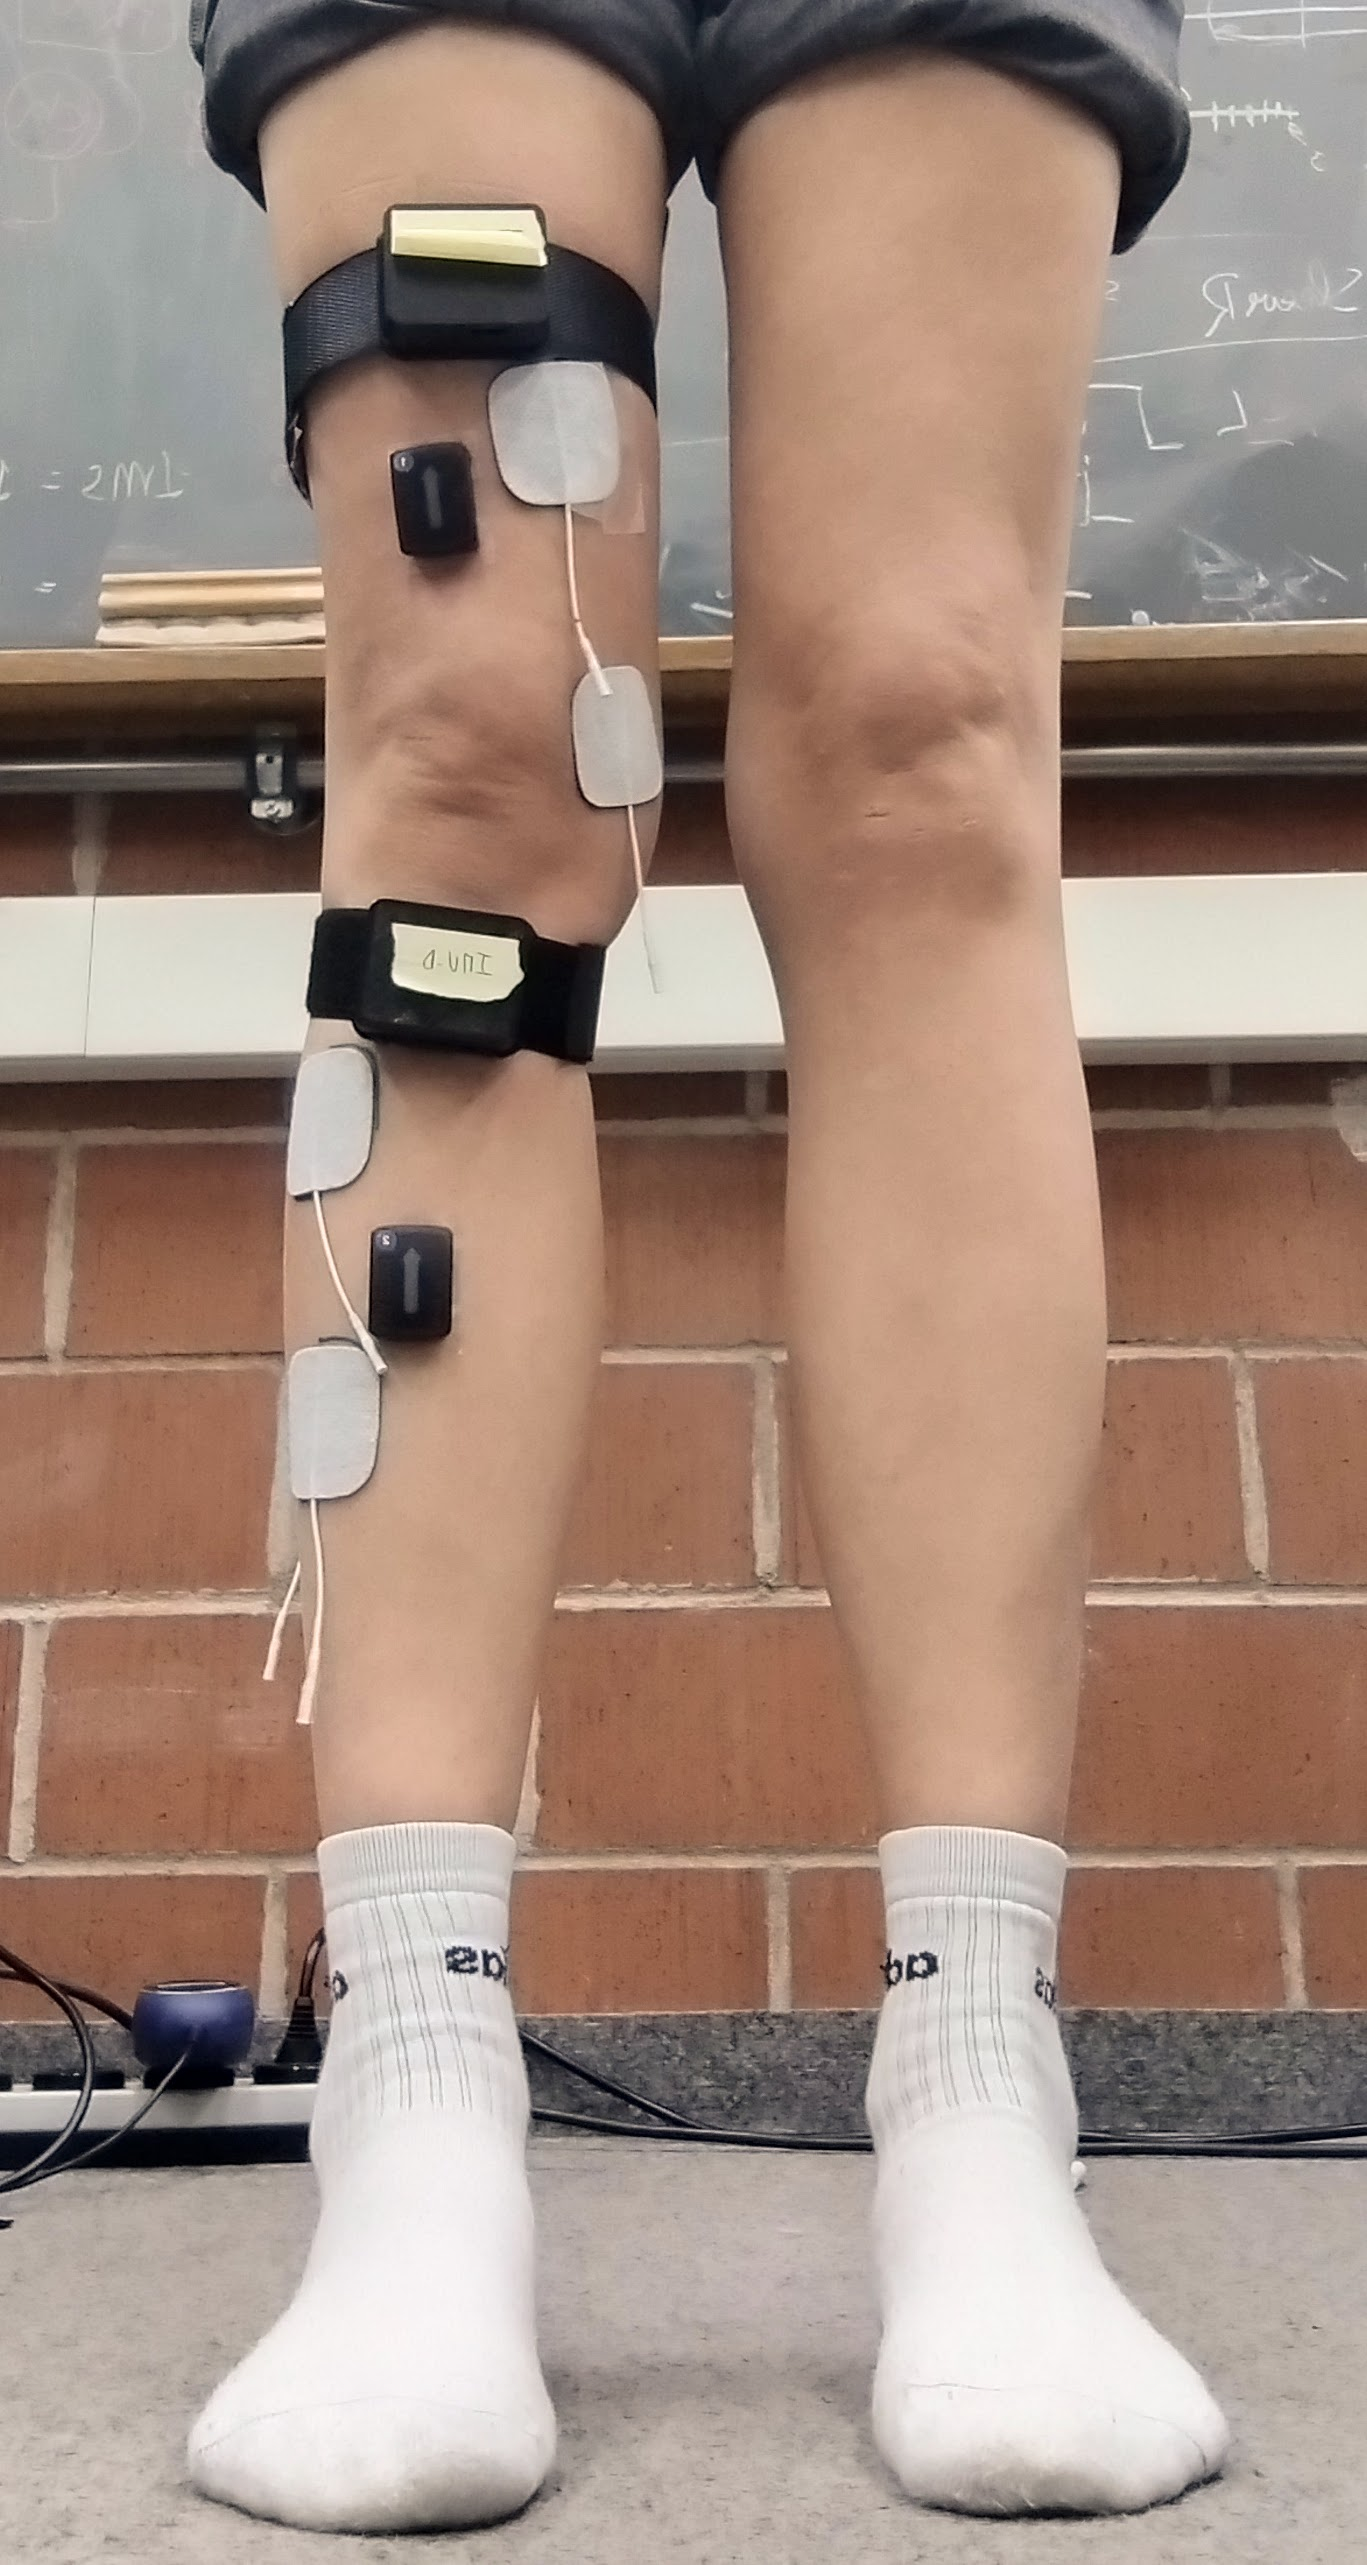
\includegraphics[width=\linewidth]{images/delsyssetup.jpg}
    \caption{Caption}
    \label{fig:enter-label}
\end{wrapfigure}

The method for knee angle estimation using the In-House IMUs is described thoroughly in the methods section "Knee Angle Estimation". The method for extracting the knee angle from the Delsys sensors involved capturing the orientation data that the sensors provide already having used sensor fusion. The relative orientation between the two sensors is then computed by taking the inverse of the thigh sensor's rotation and applying it to the shank sensor's rotation. This relative rotation is then converted to Euler angles from which the rotation about the x-axis is extracted:
\begin{equation}
    \theta_{\text{knee}} = \text{Euler}_x \left( \mathbf{q}_{\text{thigh}}^{-1} \otimes \mathbf{q}_{\text{shank}} \right)
\end{equation}

The validation experiment consisted of mounting the Delsys IMUs and In-House IMUs on the thigh and shank as seen in figure \todo{ref}. The subject was then instructed to sit and move their leg from resting on the ground at approximately a 90 degree angle to resting it on a chair at a full extension, meaning approximately zero degrees. In order to compare the two estimates, the computed knee angles were synchronized and compared over a shared time range. Linear interpolation was applied to both datasets to align them temporally, accounting for potential differences in sampling rates and starting times. The synchronized data allows for a direct comparison as can be seen in figure \ref{fig:t11}. 

\subsection{Algorithm Evaluation}
Four main methods were selected for evaluation based on their applicability, robustness and ease of implementation. These were the complementary filter, the Mahony filter, the Madgwick filter and finally the Extended Kalman Filter.

The first method considered was the complementary filter, which offers the simplest approach. This filter relies on a weighted combination of data from accelerometers and gyroscopes, leveraging their complementary characteristics. Low-frequency data from the accelerometer provides reliable long-term orientation estimates due to the absence of drift, while high-frequency data from the gyroscope captures rapid angular changes with greater precision. By blending these data streams, the complementary filter achieves effective orientation estimation without the need for complex calculations. Its primary strengths lie in its simplicity, ease of implementation, and extremely low computational cost, making it an appealing choice for systems with limited resources. However, the complementary filter is less robust than the Mahony filter in scenarios involving dynamic motion. External accelerations, such as those caused by foot strikes, can corrupt accelerometer data and lead to errors. \todo{sources}

The second method considered was the Mahony filter, a computationally efficient sensor fusion algorithm widely used for orientation estimation. This filter utilizes a proportional-integral (PI) controller framework to combine data from gyroscopes, accelerometers, and, optionally, magnetometers. The proportional term corrects instantaneous orientation errors by aligning the measured accelerations with expected gravitational vectors, while the integral term addresses the accumulated drift of the gyroscope data over time. The Mahony filter is particularly valued for its simplicity and ability to effectively compensate for gyroscopic drift without demanding extensive computational resources. However, its reliance on static assumptions about the accelerometer’s measurement of the gravity vector can limit its performance in highly dynamic environments. This potential limitation was a significant consideration given the dynamic nature of this application. \todo{sources}

The third method evaluated was the Madgwick filter, which distinguishes itself from the Mahony and complementary filters by its use of a gradient-descent-based algorithm for orientation estimation. Like the Mahony filter, the Madgwick filter combines gyroscope and accelerometer data to produce robust orientation estimates, but its correction step involves aligning the predicted and measured gravity vectors using a gradient descent optimization. This approach provides a more direct correction for gyroscopic drift and is particularly well-suited to environments where accelerometer data may be noisy. The Madgwick filter is computationally efficient and designed specifically for low-cost, noisy IMUs, making it comparable to the Mahony filter in terms of resource requirements. However, its use of gradient descent allows for potentially faster convergence and more precise correction in dynamic conditions. Unlike the complementary filter, both the Mahony and Madgwick filters model gyroscopic drift explicitly, making them more suitable for long-term orientation tracking.

The fourth method, the Extended Kalman Filter (EKF), offers a more sophisticated sensor fusion approach by combining noisy sensor data with a system model within a probabilistic framework. The EKF predicts orientation using gyroscope data and refines it by comparing predicted and measured values from the accelerometer. This allows the EKF to handle both short-term dynamics and long-term drift, making it theoretically robust. However, the EKF is computationally intensive, requiring matrix operations and Jacobian calculations, which introduce latency and make it unsuitable for real-time applications with limited resources. Additionally, it is sensitive to initialization errors, sensor misalignment, and external accelerations, such as foot strikes, which can degrade performance. Compared to the Mahony and Madgwick filters, which are tailored for efficient real-time use in noisy and dynamic environments, the EKF prioritizes theoretical accuracy but is impractical for this project's constraints.

After evaluating the four methods, the Madgwick filter was chosen as the best option for this project due to its balance of accuracy, robustness, and computational efficiency. The complementary filter, while simple and efficient, lacked explicit drift correction and was prone to errors in dynamic conditions, making it unsuitable for accurate knee angle estimation. The Mahony filter provided better drift correction but would likely have struggled in highly dynamic environments due to its reliance on static assumptions about accelerometer measurements. The Extended Kalman Filter, though theoretically robust, was too computationally intensive and sensitive to initial conditions for real-time use in this project. The Madgwick filter stood out for its ability to correct gyroscopic drift effectively using gradient descent, making it more precise and reliable in noisy and dynamic conditions while remaining computationally efficient. These factors made it the most practical and reliable choice for this application.

\subsection{Implementation}
\subsubsection{Wireless IMU Integration}
In order to access the IMU data streams, connections were set up to the LSL streams emitted by the IMUs. Each device was configured as an independent source, transmitting real-time data. Modular code using threading was developed to ensure that the connection setup, data acquisition and processing could handle multiple IMUs simultaneously. The use of multithreading ensured that data from each IMU could be processed concurrently and thereby did not create delays in the real-time system. 

\begin{figure} [h]
    \centering
    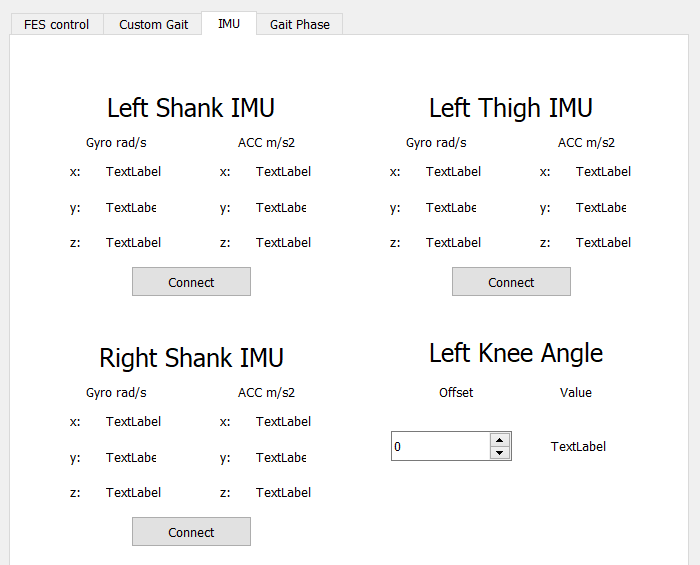
\includegraphics[width=0.7\linewidth]{images/imugui1.png}
    \caption{Graphical User Interface for visualizing IMU values and connecting new IMUs}
    \label{fig:imugui}
\end{figure}

A new tab for the GUI was also created in order to visualize the data in real time and allow the user to choose which IMUs to connect. A screenshot of the GUI can be seen in figure \ref{fig:imugui}. There were four IMUs available at the laboratory designated A, B, C and D, in the code these IMUs are assigned as either left or right, shank or thigh IMUs. This mapping may easily be changed, which is useful when working with wireless IMUs that need regular charging. The connect button triggers creation of a new instance of the IMU class and a new thread on which the data is processed and sent back to be visualized in the "TextLabel" fields.

\subsubsection{Madgwick Filter for Knee Angle Estimation}
The Madgwick filter is a gradient-descent-based orientation estimation algorithm. It provides a computationally efficient framework to estimate the orientation based on using gyroscope data for the prediction step and accelerometer data for the correction step. 

The Madgwick filter would be implemented on the thigh and shank IMUs individually. The implementation outlined here is adapted from the original internal report by S. Madgwick  \cite{madgwick_ecient_nodate} and the documentation of the AHRS implementation \cite{noauthor_madgwick_nodate}. In the Madgwick filter the orientation of the sensor frame relative to the earth frame is represented as a quaternion \( \mathbf{q_{\omega , t}} \):
\[
\mathbf{q_{\omega , t}} = 
\begin{bmatrix}
q_w & q_x & q_y & q_z
\end{bmatrix}^T
\]
where \( q_w \) is the scalar part, and \( q_x, q_y, q_z \) are the vector components.
\newline

\paragraph*{Prediction step: Integration of Angular Velocity}

The orientation quaternion is predicted by numerically integrating the quaternion derivative 
\(
\dot{\mathbf{q}}_t = \frac{1}{2} \mathbf{q}_{t-1} \otimes \boldsymbol{\omega}_t
\) as:
\[
\mathbf{q}_{\omega, t} = \mathbf{q}_{t-1} + \dot{\mathbf{q}}_{\omega, t} \Delta t
\]
\[
\mathbf{q}_{\omega, t} = \mathbf{q}_{t-1} + \frac{1}{2} \left( \mathbf{q}_{t-1} \otimes \mathbf{S}\boldsymbol{\omega}_t \right) \Delta t
\]
where \( \Delta t \) is the sampling period and 
\(
\mathbf{S}\boldsymbol{\omega} = 
\begin{bmatrix}
0 & \omega_x & \omega_y & \omega_z
\end{bmatrix}
\)
is the tri-axial angular rate, in rad/s, measured in the sensor frame and represented as a pure quaternion. For a more detailed explanation on orientation estimation based solely on angular rate and quaternion kinematics the reader is referred to \cite{sola_quaternion_2017}.
\newline

\paragraph*{Correction step: Gradient Descent}

To correct for gyroscope drift, the Madgwick filter uses accelerometer data to align the predicted gravity vector with the measure gravity vector. The objective function minimizes the error between the two:
\[
f(\mathbf{q}) = \mathbf{q}^* \otimes \mathbf{g} \otimes \mathbf{q} - \mathbf{a}
\]

Where  \( \mathbf{q}^* \) is the conjugate of the predicted quaternion. The reference gravity vector in the Earth frame is \(\mathbf{g} = [0, 0, 0, 1].\) and the normalized accelerometer measurement is
    \(
    \mathbf{a} = [0, a_x, a_y, a_z].
    \)

The gradient of the objective function is computed as:
\[
\nabla f(\mathbf{q}) = \mathbf{J}^T f(\mathbf{q})
\]

where \( \mathbf{J} \) is the Jacobian matrix of the objective function.

It follows that the corrected quaternion is updated using a gradient descent step given by:
\[
\mathbf{q}_{k+1} = \mathbf{q}_k - \mu \frac{\nabla f(\mathbf{q})}{\|\nabla f(\mathbf{q})\|}
\]

where \( \mu \) is the step size (gain), which controls the convergence rate.
\newline

\paragraph*{Application to Knee Angle Estimation}

 The algorithm is used to estimate the orientation of each IMU relative to the Earth frame, yielding quaternions \( \mathbf{q}_{\text{thigh}} \) and \( \mathbf{q}_{\text{shank}} \). The knee angle is then computed as the relative orientation between the two IMUs calculated as:
\[
\mathbf{q}_{\text{relative}} = \mathbf{q}_{\text{shank}} \otimes \mathbf{q}_{\text{thigh}}^*,
\]
where \( \mathbf{q}_{\text{thigh}}^* \) is the conjugate of \( \mathbf{q}_{\text{thigh}} \).

The knee angle \( \theta \) is derived from the relative orientation quaternion:
\[
\theta = \arccos{\left( 2q_w^2 - 1 \right)},
\]
where \( q_w \) is the scalar component of \( \mathbf{q}_{\text{relative}} \).

\paragraph*{Software Realization}
In order to implement the Madgwick filter the AHRS library was utilized \cite{noauthor_madgwick_nodate} and built upon. In order to be used for knee angle estimation some output functions needed to be added to the library and the equations outlined in the "application to knee angle estimation" had to be added. The knee angle estimation was also threaded such that it would not produce delays in the main thread or the closed loop threads. 

A thorough delay logging was also implemented in order to validate that the filtering and calculations did not introduce too large delays that would introduce issues in the closed loop control. \todo{insert delay results}

\subsection{Results}
\begin{figure} [H]
    \centering
    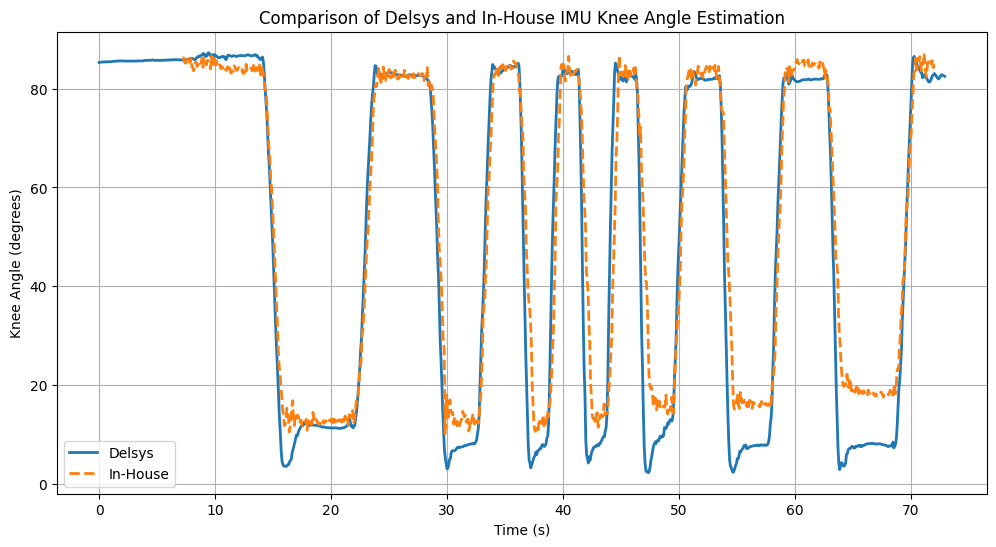
\includegraphics[width=0.95\linewidth]{images/T11_betterplotting.png}
    \caption{}
    \label{fig:t11}
\end{figure}

The results show that the adapted Madgwick filter does a good job of estimating the knee angle. However we see some slight drift, even though the Madgwick filter should in theory be robust to drift. It is however worth noting here that there are some clear inaccuracies in the Delsys derived knee angle as well. Specifically we observe that there is a valley in the calculated knee angle followed by a flattening out of the curve when the knee is extended, this does not reflect the actual movement that the subject performs. The ideal performance of the IN-House developed knee angle estimation is therefore not necessarily an exact replication of the Delsys curve. The In-House algorithm does not seem to have this same artifact.

\subsection{Discussion}
The results of the knee angle stimulation demonstrate that the In-House IMU-based estimation method, which utilizes an adapted Madgwick filter, performs effectively in estimating knee joint angles during movement. However, slight drift in the estimation was observed, despite the theoretical robustness of the Madgwick algorithm to such errors. This drift could be attributed to several factors the first of which is that the way in which the algorithm is implemented assumes that the local coordinate axes of the IMUs are perfectly aligned with the anatomical knee joint axis. Any misalignment introduces errors in the computed knee angle, as the algorithm assumes that the relative orientation of the two IMUs reflects the hinge joint's motion accurately.

\begin{figure}
    \centering
    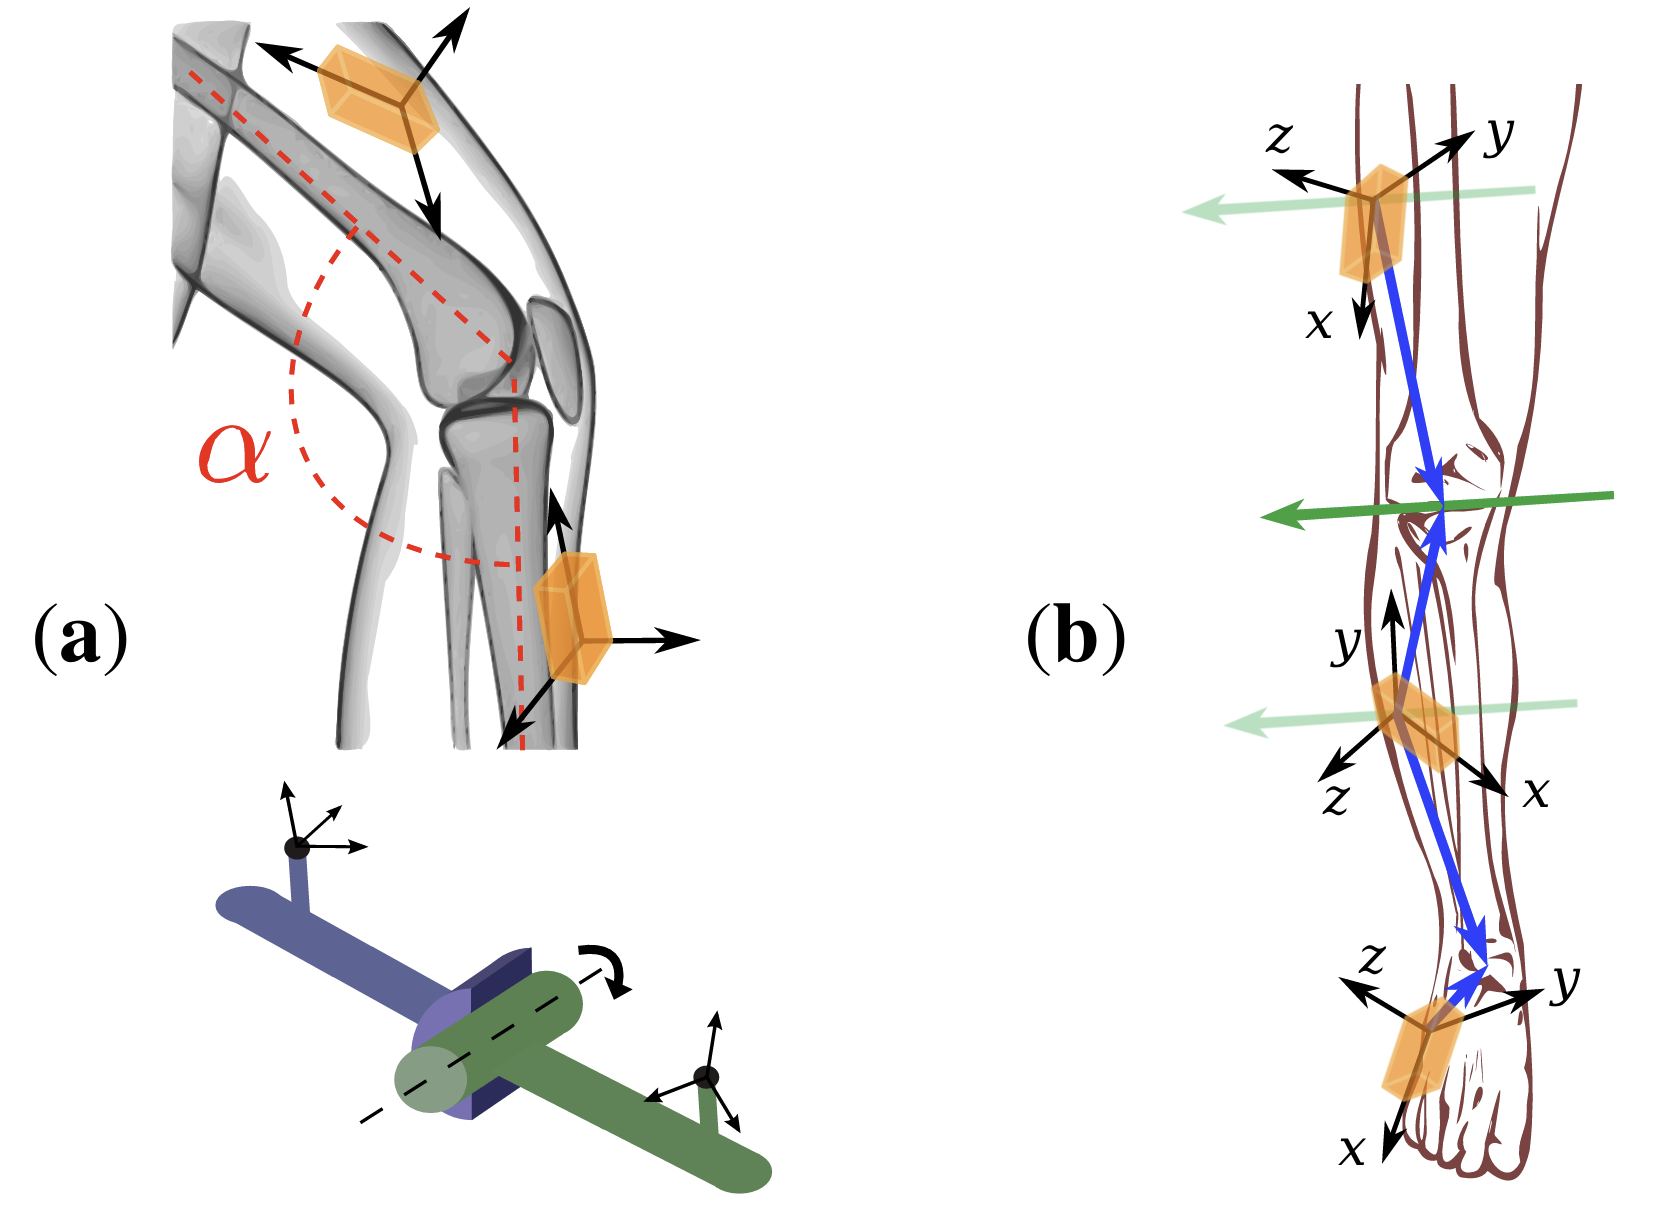
\includegraphics[width=0.75\linewidth]{images/kneeOrientation.png}
    \caption{\textbf{a)} Local sensor coordinate axes are not aligned with the physiological axes and planes by which the joint angle, \(\alpha\), is defined \textbf{b)} The coordinates of the joint axis direction (green arrows) and the joint position (blue arrows) in the local coordinate system of the sensors \cite{seel_imu-based_2014}}
    \label{fig:enter-label}
\end{figure}

This issue is further compounded by the possible shifting of the IMUs over time. This poses issues since the initial offset between the IMUs is assumed to be accurately calibrated and constant throughout the session. Additionally the Madgwick filter is not capable of accounting for changes in sensor alignment over time, leading to possible inaccuracies if the IMUs are not secured well enough.

Another related challenge is the implicit assumption that the IMUs are do not experience significant external forces beyond those caused by the forward motion of the leg and gravity. In practice however, accelerometer readings can be affected by transient forces such as those that occur during foot strikes. These forces may introduce noise into the orientation estimation process, specifically in the correction step of the Madgwick filter, where accelerometer data is used to align the estimated gravity vector with the measured gravity vector.

Finally there is room for improvement with regards to the validation process itself. The Delsys derived knee angle, although likely more accurate than the In-House version since it has inbuilt sensor fusion algorithms for orientation estimation, is still using IMUs in order to estimate the angle. In order to benchmark in a better manner a goniometer sensor should be used instead or an even more robust sensor system. This could for example be the Xsens system used for validation of the open loop sequence which outputs knee angles without any additional processing necessary, but was regretfully not available during the period in which the knee angle estimation method was to be validated.. 

\subsection{Further Work}
One of the challenges encountered when implementing a knee angle estimation algorithm is the need for alignment of the sensor frames to the relevant body segments. Although this is in effect implemented in the Madgwick filter by .... 


Future work could explore the integration fo real-time alignment correction mechanisms, potentially leveraging additional data sources, such as magnetometers to monitor and adjust sensor alignment continuously.

Further work could involve implementing motion segmentation algorithms to differentiate between periods of high and low dynamic activity allowing the algorithm to weigh accelerometer corrections more effectively.

not implemented here a possible further development would be to implement a sensor-to-segment alignment. Such algorithm can generally be categorized into manual alignment, static pose estimation, functional calibration, deep learning, or some combination of these approaches \cite{rhudy_knee_2024}. For further developing this project a simple static pose such as holding still for 5 to 10s in a specified standing pose could be utilized. The accelerometers would be utilized to detect the gravity vector and thus 



\end{document}